% !TEX root = ../thesis.tex

\chapter{Relativistic effects}
\label{chapter:introreleff}

\begin{itemize}
	\item origin of relativistic effects: doppler, grav. redshift, LoS, etc
	\item why are relativistic effects important? further biasing of measurements, mimicking fnl on large scales
	\item next-gen large scale surveys, observing at higher precision etc, so more important to include correct treatment of relativistic effects
	\item galaxy overdensity with these effects, perturbation theory
	\item first order, which is sufficient for power spectrum
	\item second order, required for bispectrum. long expression? 
	\item dipole in power spectrum
	\item dipole in 2pt function
\end{itemize}

\todo[inline]{add something about rel effects and big Delta here}

\section{The dipole of the 2-point correlation function}

In this section, we will consider how relativistic effects can be isolated in the correlations of two points-- the 2-point correlation function in configuration space. The 2-point function is defined as, 
\begin{equation}
	\xi = \langle \Delta(z,\n) \Delta(z, \n') \rangle\,,
\end{equation}
and it is dependent on the triagle shape as formed by the observer and two galaxies, as illustrated in figure~\ref{fig:2ptcorr_triangle_bonvin}. 
\todo[inline]{do primed vectors need a bold prime?}
\todo[inline]{do I need to spell figure with a capital F?}
\todo[inline]{remake figure of triangle (illustrator)}
\begin{figure}[ht]
	\centering
	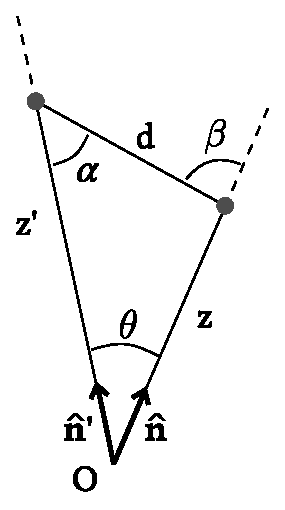
\includegraphics[width=0.3\textwidth]{fig/bonvin_triangle2pt.eps}
	\caption{Illustration of the triangle which is formed by the observer O, and two galaxies which are located at the positions $(z,\n)$ and $(z,\n')$. $\theta$ is the separation angle between the two directions of observation, $\beta$ is the angle between $\n$ and the galaxies' directional separation vector $\bm{N}$, and $d$ denotes the comoving distance between the two galaxies. Taken from~\cite{Bonvin:2014owa}.}
	\label{fig:2ptcorr_triangle_bonvin}
\end{figure}
The 2-point correlation function can be expressed as a function of three quantities, where there is a choice of coordinate systems. One such choice is to write $\xi(z, z', \theta)$, which has the advantage of being the system in which the measurements are performed, and as such it is directly observable and not reliant on cosmological assumptions. Another valid choice is to express the 2-point correlation function as dependent on parameters $(z,d,\beta)$, where $d$ denotes the comoving distance between the two galaxies, and $\beta$ here is the angle between $\n$ and $\bm{N}$, the latter vector corresponding to the galaxies' separation vector. An advantage of this choice of coordinates is that it exploits in a natural way the symmetries of the different contributions to the observed galaxy number count $\Delta_g$. However, a disadvantage of this approach is that it requires one to translate the redshifts and separation angle of the galaxies into the comoving distance $d$ and the angle $\beta$, which inconveniently relies on a choice for background cosmology. 

In this coordinate system, the density term is independent of $\beta$, and takes an extremely simple form due to statistical homogeneity and isotropy of the primordial density fluctuations, 
\begin{equation}
	\xi^\mathrm{dens} = \langle b(z) \delta(z,\n) b(z') \delta(z', \n') \rangle\,,
\end{equation}
which dpeends only on the comoving separation distance $d$ of the galaxies, and on redshift $z$. 
RSD however depend explicitly on $\beta$. Including RSD in the correlation function, 
\begin{equation}
	\xi^\mathrm{RSD} = \left\langle \left( b(z) \delta(z,\n) - \frac{1}{\cH(z)} \partial_r (\bm{V} \cdot \n) \right) \left( b(z') \delta(z', \n') - \frac{1}{\cH(z')} \partial_{r'} (\bm{V} \cdot \n') \right) \right\rangle\,,
\end{equation}
it is sensitive to the orientation of the galaxy pair with respect to the observer. It can be shown that in the distant-observer approximation \todo{define the distant-observer approximation}, this dependence on $\beta$ is very simple. The cross-correlation between density and velocity generates a quadrupole modulation, which is proportional to $P_2(\cos\beta)$ ($P_\ell$ being the Legendre polynomials), whereas velocity-velocity autocorrelation generates a hexadecapole which is proportional to $P_4(\cos\beta)$. 


\iffalse


Relativistic effects in galaxy number counts at first and second order\todo{write intro why relativistic effects important}

copypastes of old introductions in papers:

The Fourier galaxy bispectrum is complex, with the imaginary part arising from leading-order relativistic corrections, due to Doppler, gravitational redshift  and related line-of-sight effects  in redshift space. The detection of the imaginary  part of the bispectrum is potentially a smoking gun signal of relativistic contributions. Long-mode relativistic effects couple to  short-mode Newtonian effects in the galaxy bispectrum, but not in the galaxy power spectrum. This is  the basis for detectability of relativistic effects in the bispectrum of a single galaxy survey, whereas the power spectrum requires multiple galaxy surveys to detect the corresponding signal.

The bispectrum of number count fluctuations in redshift space will become an increasingly important complement to the power spectrum in the extraction of cosmological information from galaxy surveys, 
{in the measurement of {clustering} bias parameters and in the breaking of degeneracies between the clustering amplitude and growth rate.}
Analysis of the Fourier galaxy bispectrum is already well advanced for existing survey data (e.g \cite{Gil-Marin:2016wya,Sugiyama:2018yzo}) and for mock data of future surveys (e.g. \cite{Karagiannis:2018jdt,Yankelevich:2018uaz,Oddo:2019run,Sugiyama:2019ike}). 

We investigate the detectability of leading-order relativistic effects in the bispectrum of future 21cm intensity  mapping surveys. The relativistic signal arises from Doppler and other line-of-sight effects in redshift space. In the power spectrum of a single tracer, these effects are suppressed by a factor $\cH^2/k^2$. By contrast, in the bispectrum the relativistic signal couples to short-scale modes, leading to
an imaginary contribution that scales as $\cH/k$, thus increasing the possibility of detection.
Previous work has shown that this relativistic signal is detectable in a Stage IV H$\alpha$ galaxy survey. 
{We show that the signal is also detectable by next-generation  21cm intensity maps, but typically with a lower signal-to-noise, due to foreground and telescope beam effects.}


{Next-generation galaxy surveys will allow for precision measurements of the  bispectrum, bringing new information to improve constraints on cosmological parameters and to break some of their degeneracies (see e.g. \cite{Scoccimarro:2015bla,Tellarini:2016sgp, Gil-Marin:2016wya,  Slepian:2016kfz,Gagrani:2016rfy, Sugiyama:2018yzo,Desjacques:2018pfv,Child:2018klv, Yankelevich:2018uaz, Schmit:2018rtf,DiDio:2018unb,Gualdi:2019ybt,Sarkar:2019ojl,Chudaykin:2019ock,Oddo:2019run, Sugiyama:2019ike,Philcox:2019hdi,Durrer:2020orn,Montanari:2020uez}). 

These surveys will typically probe very large volumes in the Universe, including ultra-large scales ($k\lesssim k_{\mathrm{eq}} \sim 0.01\;\mathrm{Mpc}^{-1}$), which facilitates the detection of, or precision constraints on, primordial non-Gaussianity \cite{Tellarini:2015faa,Watkinson:2017zbs,Majumdar:2017tdm,Karagiannis:2018jdt,Karagiannis:2019jjx,Bharadwaj:2020wkc}
and relativistic effects
\cite{Kehagias:2015tda,Umeh:2016nuh, DiDio:2016gpd, Jolicoeur:2017nyt,Bertacca:2017dzm,Jolicoeur:2017eyi,Koyama:2018ttg,Clarkson:2018dwn,Maartens:2019yhx,Jeong:2019igb}.
 
Redshift-space distortions (RSD) are the dominant observational effect on the number counts or brightness temperature at first and second order in perturbations. There are local relativistic corrections to standard RSD, arising from Doppler and other line-of-sight gradient terms, together with their couplings.  In Fourier space, the leading-order corrections  scale as $\i(\cH/k)$. In the tree-level power spectrum of a single tracer, the only nonzero contribution from these Doppler-type effects is from their square, since the power spectrum is necessarily real. As a result, the Doppler-type effects are further suppressed in the auto-power spectrum, scaling as  $(\cH/k)^2$. 

The tree-level bispectrum of a single tracer is not forced to be real and it couples Doppler-type effects with the standard (`Newtonian') density + RSD term. Consequently, the leading-order relativistic contribution to the bispectrum scales as i\,$(\cH/k)$. 
This means that the leading-order relativistic signal is more detectable in the bispectrum than the power spectrum, for a single tracer.
In Fourier space, the dominant relativistic effect is a purely imaginary part of the bispectrum, as shown by \cite{Clarkson:2018dwn,Maartens:2019yhx}. Our previous work \cite{Maartens:2019yhx} showed that it is detectable by a Stage IV spectroscopic galaxy survey.

%%%%%%%%%%%

Observations in large scale structure surveys pose a variety of challenges. As opposed to CMB observations, in which in great detail temperature fluctuations can be measured and mapped, LSS surveys have the downside that one observes galaxies and not the underlying density field. Since galaxies are a biased tracer of the underlying density field, this in itself imposes the problem of how galaxy clustering biases measurements. Furthermore, there are various sources of non-linearities in galaxy clustering, which give rise to non-trivial higher order correlations aside from the power spectrum. Where a purely Gaussian field is fully described by the power spectrum, that is, all statistical information about the field is contained therein and odd correlators vanish identically, in the case of non-Gaussianities the three-point correlations and higher are generated and are needed in addition to the power spectrum to describe the field at high enough accuracy. 

For a highly non-linear regime it would probably be necessary to turn to full numerical simulations for an analysis, but in the intermediate, weakly non-linear regime, higher order perturbation theory can be used for our analysis. In this chapter I will discuss the relativistic effects on galaxy number counts at first and second order.  

In a typical galaxy survey, the observer looks down the past lightcone and observes some number of galaxies $\diff N$, which are above some threshold luminosity $L$, in a redshift interval $\diff z$ and within an element of solid angle $\diff \Omega_o$, about direction of observation $\n$. 

The fractional perturbation of observed number counts $\Delta_g$ is defined by 
\begin{equation}
	\frac{\diff N(z, \n, > \ln L)}{\diff z \diff \Omega_o} = \frac{\chi^2(z)}{(1 + z)^4 \cH(z)} \bar{\N}(z, > \ln L) \left[ 1 + \Delta_g(z, \n, >\ln L)\right], 
\end{equation}

where $\cH$ is the conformal Hubble rate, $\chi$ is the comoving line-of-sight distance, and $\bar{\N}$ is the background magnitude-limited number density of sources. The dependence of $\Delta_g$ on $\ln L$ will be suppressed for brevity. Expanding $\Delta_g$ up to second order in perturbation theory as follows, 
\begin{equation}
	\Delta_g(z,\n) = \Delta_g^\on(z,\n) + \frac{1}{2} \left[ \Delta_g^\tw(z,\n) - \langle \Delta_g^\tw (z,\n)\rangle \right],
\end{equation}
subtracting off the average value of $\Delta_g^\tw$ to ensure that $\langle \Delta_g \rangle = 0$.

\section{Relativistic effects in LSS}

\section{First order in perturbation theory}

see title

\section{Second order in perturbation theory}

see title again 

\section{Relativistic contributions to the galaxy power spectrum}



\section{Relativistic contributions to the galaxy bispectrum}

\fi